\section{Result}

From the posterior distribution, we know that the probability of legislature have$Pr(liec > 0) = 0.89$ close to significant.

\begin{table}[ht]
\centering
\begin{tabular}{rrrrrr}
  \hline
 & mean & 2.5\% & 97.5\% & Pr( $>$ 0) & Pr( $<$ 0) \\ 
  \hline
legislature & 0.48 & -0.29 & 1.25 & 0.89 &  \\ 
  log(GDP percap) & -0.39 & -1.31 & 0.52 &  & 0.81 \\ 
  log(GDP) & 0.37 & -0.19 & 0.92 & 0.91 &  \\ 
  resource (\%GDP) & -0.01 & -0.04 & 0.02 &  & 0.78 \\ 
  military exp (\%GDP) & -0.04 & -0.27 & 0.19 &  & 0.63 \\ 
  regime duration & 0.02 & -0.03 & 0.08 & 0.78 &  \\ 
  military regime & 2.10 & -1.79 & 5.84 & 0.86 &  \\ 
  personal regime & 1.60 & -1.65 & 4.89 & 0.83 &  \\ 
  party regime & 3.09 & -0.10 & 6.31 & 0.97 &  \\ 
   \hline
\end{tabular}
\caption{Hierarchical model parameter estimates}
\label{tab:hierarchical_estimate}
\end{table}

\begin{figure}[ht]
    \centering
    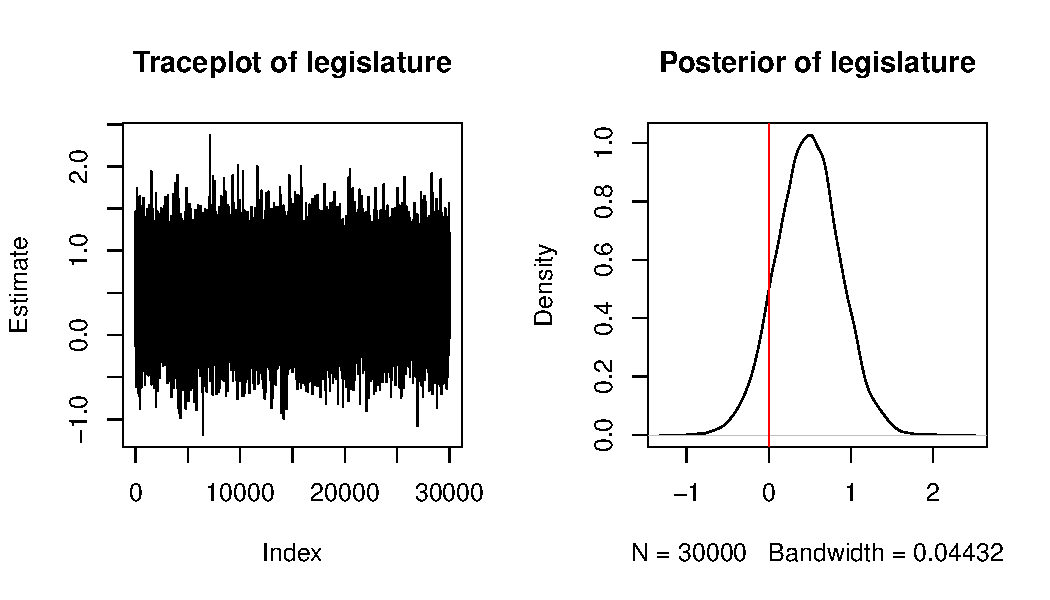
\includegraphics[width=\textwidth]{../fig/mcmc_legis}
    \label{fig:mcmc_legis}
\end{figure}
